%                                                                 aa.dem
% AA vers. 9.1, LaTeX class for Astronomy & Astrophysics
% demonstration file
%                                                       (c) EDP Sciences
%-----------------------------------------------------------------------
%
%\documentclass[referee]{aa} % for a referee version
%\documentclass[onecolumn]{aa} % for a paper on 1 column  
%\documentclass[longauth]{aa} % for the long lists of affiliations 
%\documentclass[letter]{aa} % for the letters 
%\documentclass[bibyear]{aa} % if the references are not structured 
%                              according to the author-year natbib style

%
\documentclass{aa}  

%
\usepackage{graphicx}
%%%%%%%%%%%%%%%%%%%%%%%%%%%%%%%%%%%%%%%%
\usepackage{txfonts}
%%%%%%%%%%%%%%%%%%%%%%%%%%%%%%%%%%%%%%%%
%\usepackage[options]{hyperref}
% To add links in your PDF file, use the package "hyperref"
% with options according to your LaTeX or PDFLaTeX drivers.
%

\usepackage{color}
\newcommand{\hw}[1]{\textcolor{red}{HW: #1}}
\newcommand{\todo}[1]{\textcolor{green}{TODO: #1}}

\begin{document} 


   \title{Simulating the Universe from the Cosmic Microwave Background to Today}

   \subtitle{}

   \author{A. Martins
          \inst{1}
          }

   \institute{Institute of Theoretical Astrophysics, University of Oslo,
              Sem Sælands vei 13, 0371 Oslo\\
              \email{a.i.s.martins@astro.uio.no}
             }

   \date{}

% \abstract{}{}{}{}{} 
% 5 {} token are mandatory
 
  \abstract
  % context heading (optional)
  % {} leave it empty if necessary  
   {}
  % aims heading (mandatory)
   {We have simulated the large scales of the universe, as well as the recombination and reionisation processes.}
  % methods heading (mandatory)
   {We use a Markov chain Monte Carlo to predict the densities of the different components of the Universe, as well as solving ordinary differential equations using a fourth-order Runge-Kutta method.}
  % results heading (mandatory)
   {We find the times of radiation-matter and matter-dark energy equality to be $x=-8.1319$ and $x=-0.25582$. Recombination happens at $x=-7.0$, while recombination happens at $x=-2.2$.}
  % conclusions heading (optional), leave it empty if necessary 
   {}

   \keywords{CMB, Hubble constant, MCMC, Recombination, Reionisation}

   \maketitle
%
%-------------------------------------------------------------------

\section{Introduction}

\subsection{Background Cosmology}
Since its discovery in 1964 \citep{1965ApJ...142..419P, 1965ApJ...142..414D}, the Cosmic Microwave Background (CMB) is still one of the biggest topics of interest in Cosmology today.
As such, we are interested in simulating its power spectrum in order to fully understand how it looks like and how inflation might have looked like. It is useful to start with what the Universe looks like on large scales.

\hw{1.1 A bit brief. A bit more context would be good here.}

\subsection{Recombination History}

A significant event in the history of the Universe is recombination. In this process, the Universe goes from being made up of a tightly coupled plasma of charged particles to having its elements combine into atoms, mostly of Hydrogen and Helium. Photons interacting with atoms is a much less common and significant occurrence than with the previously common electrons and protons, thus making it possible for photons to travel freely and so the CMB is released, letting us observe it today.

\begin{figure*}[ht]
\caption{History of the Universe. Credit: NAOJ}             
\label{fig:history}      
\centering          
\includegraphics[width=\textwidth]{report/figures/eso1620a.jpg}
\end{figure*}

\section{Theoretical Background}

\subsection{Background Cosmology}

We start by assuming that, at large scales, matter is homogeneous and isotropic. The mathematical formulation of this, i.e. the metric that describes the geometry of the Universe at large scales is given by the Friedmann–Lemaître–Robertson–Walker (FRLW) metric:
\begin{equation}
ds^2 = -dt^2 + a^2(t)(dx^2 + dy^2 + dz^2),
\end{equation}
where $a(t)$ is the scale factor of the Universe, a measure for the rate of its expansion.

We are interested in learning about the densities of the different components of the Universe at different points in time, from the Cosmic Microwave Background until the present day. The $\Lambda$CDM model assumes that the Universe is composed of matter (baryons\footnote{Baryons in this context refers to all "normal" matter, i.e. quarks, leptons (not including neutrinos for our purposes) and combinations of them.} and cold, dark matter), radiation (photons and neutrinos) and dark energy. Another important notion for our model is that of curvature, which we already implicitly assumed to be 0 in the above equation, i.e. we are assuming a flat Universe. These components come together in the Friedman equation, which relates their density evolution to the expansion of the Universe:
\begin{equation}
H(a) = H_0 \sqrt{\Omega_{M0}a^{-3} + \Omega_{R0}a^{-4} + \Omega_{k 0} a^{-2} + \Omega_{\Lambda 0}},
\end{equation}
where $H(a)$ is the so-called Hubble parameter and $H_0$ is the Hubble constant, measured experimentally today to be around 68.3 km s$^{-1}$ Mpc$^{-1}$ \citep{Kozmanyan_2019}. Each $\Omega_{i0}$ represents the density of one of the above-mentioned components in the present day, now explicitly including curvature $k$, and $\Omega_{M0} = \Omega_{b0} + \Omega_\text{CDM0}, \Omega_{R0} = \Omega_{\gamma0} + \Omega_{\nu0}$. The densities for photons and neutrinos today are given by
\begin{align}
\Omega_{\gamma 0} &= 2\cdot \frac{\pi^2}{30} \frac{(k_bT_{\rm CMB 0})^4}{\hbar^3 c^5} \cdot \frac{8\pi G}{3H_0^2},\\
\Omega_{\nu 0} &= N_{\rm eff}\cdot \frac{7}{8}\cdot \left(\frac{4}{11}\right)^{4/3}\Omega_{\gamma 0},
\end{align}
whereas the densities for baryons and cold, dark matter are assumed to be, respectively, 0.05 and 0.267, the values given by \cite{2020}. The densities of all the components need to, of course, add up to one. We then find that 
$\Omega_{\Lambda 0} = 1 - (\Omega_{b 0}+\Omega_{\rm CDM 0}) - (\Omega_{\gamma 0} + \Omega_{\nu 0}) - \Omega_{k 0}$, where, assuming a flat universe, $\Omega_{k 0} = 0$.

We can get the component densities for different scale factors from
\begin{equation}
\label{eq:omegas}
\begin{aligned}
\Omega_{k}(a) &= \frac{\Omega_{k0}}{a^2H(a)^2/H_0^2}\\
\Omega_{\rm CDM}(a) &= \frac{\Omega_{\rm CDM 0}}{a^3H(a)^2/H_0^2} \\
\Omega_b(a) &= \frac{\Omega_{b 0}}{a^3H(a)^2/H_0^2} \\
\Omega_\gamma(a) &= \frac{\Omega_{\gamma 0}}{a^4H(a)^2/H_0^2} \\
\Omega_{\nu}(a) &= \frac{\Omega_{\nu 0}}{a^4H(a)^2/H_0^2} \\
\Omega_{\Lambda}(a) &= \frac{\Omega_{\Lambda 0}}{H(a)^2/H_0^2}.
\end{aligned}
\end{equation}

It is handy to explore the Hubble parameter equations before introducing some new notions. In particular, a useful quantity is the scaled Hubble parameter $\mathcal H = aH$. Differentiating this with respect to $x = \log a$ and denoting the derivative with respect to $x$ as ', we have
\begin{align}
    \mathcal H' &= \frac{d\mathcal H}{dx} = \frac{da}{dx}\frac{d\mathcal H}{da}\\ 
    &= a\left( H(a) + \frac{1}{2}\frac{aH_0^2}{ H(a)} (-3\Omega_{M0} a^{-4} - 4\Omega_{R0}a^{-5}-2\Omega_{k0}a^{-3})\right)\\
    &= \mathcal H(x) +\frac{1}{2}\frac{(e^xH_0)^2}{\mathcal H(x)}(-3\Omega_{M0} e^{-3x} - 4 \Omega_{R0}e^{-4x}-2\Omega_{k0}e^{-2x}).
\end{align}

Differentiating once more, we get
\begin{alignat*}{2}
    \mathcal H'' &= \frac{d^2\mathcal H}{dx^2}&&\\ 
    &= \mathcal H'\Bigg(1-&&\frac{1}{4}\left(\frac{e^xH_0}{\mathcal H(x)}\right)^5\\
    & &&(3\Omega_{M0}e^{-3x}+4\Omega_{R0}e^{-4x}+2\Omega_{k0}e^{-2x})^2\\
    & &&(9\Omega_{M0}e^{-3x}+16\Omega_{R0}e^{-4x}+4\Omega_{k0}e^{-2x})\Bigg)
\end{alignat*}

It is now useful to define the notion of conformal time $\eta$, the distance the light has traveled since the Big Bang, taking into account the expansion of the Universe. A differential equation for $\eta$ can be written as
\begin{align}
\frac{d\eta}{dx} = \frac{da}{dx}\frac{d\eta}{da} = \frac{c}{\mathcal{H}}.
\end{align}

From this, follow the definition of the co-moving distance $\chi$, the distance between the observer and a measurable quantity:
\begin{align}
\chi = \eta_0 - \eta
\end{align}

For a flat Universe, we can define the luminosity distance, i.e. given the intrinsic luminosity of a source and its flux, the distance to the source is

\begin{equation}
    d_L = \frac{\chi}{a}.
\end{equation}

\hw{Eq. 11 is for a flat Universe only - you need this in general as this is what you implement.}

A last useful notion before we get into some deductions is that of cosmic time $t$, which is given by solving
\begin{align}
\label{eq:t-ode}
\frac{dt}{dx} = \frac{1}{H}.
\end{align}

We are now interested in looking at specific points in time, such as the points when matter and radiation had the same density and when matter and dark energy had the same density (and subsequent dominating periods), and the time when the Universe started to accelerate.

\subsubsection{Matter-Radiation Equality}

We can find the time of matter-radiation equality by equating $
\Omega_b + \Omega_{\rm CDM} = \Omega_\gamma + \Omega_{\nu}$. Using \eqref{eq:omegas}, we find that

\begin{equation}
    a = \frac{\Omega_R}{\Omega_M}.
\end{equation}

\hw{Eq. 13 It's OmegaR0 / OmegaM0 on the RHS. Same for Eq. 14}

\subsubsection{Matter-Radiation Equality}

Similarly, we find the time when matter and radiation are equally dense by equating $\Omega_b + \Omega_{\rm CDM} = \Omega_{\Lambda}$ and find that

\begin{equation}
    a = \sqrt[3]{\frac{\Omega_M}{\Omega_{\Lambda}}}
\end{equation}

\subsubsection{The Universe starts to accelerate}

In order to know when the Universe starts to accelerate, we must solve $\ddot a = 0$. By definition, $H = \dot{a}/a \Rightarrow \frac{d}{dt} \dot a = \frac{d}{dt} (aH) = \frac{d}{dt}\mathcal H$. It is not so useful to take the derivative in terms of cosmic time of the scaled Hubble parameter, but we already know what its derivative is in terms of $x$, so we can take that and get
\begin{equation}
    \ddot a = \frac{dx}{dt}\frac{d\mathcal H}{dx},
\end{equation}
where we know a handy expression for $\frac{dx}{dt}$ from \eqref{eq:t-ode} and we end up with
\begin{equation}
    \ddot a = H\mathcal{H'} = 0,
\end{equation}
where ' denotes the derivative in terms of $x$.

\hw{Eq. 16 has an analytical solution (only matter and dark energy is relevant in H at this point).}

\subsection{Recombination History}

A concept that is deeply related to the process of recombination is that of optical depth $\tau$. The optical depth is a quantity that defines the transparency of a medium to photons. If a medium has $\tau\gg1$, then we call it optically thick and no light is transmitted through it -- this was the state of the Universe before recombination. As electrons and protons combine, photons start being able to move freely without interacting with them, and the Universe's medium becomes optically thin ($\tau\ll 1$). Calculating $\tau$ will let us know when recombination happened.

The optical depth is then given by
\begin{equation}
\tau(\eta) = \int_{\eta}^{\eta_0} n_e \sigma_T a d\eta',
\end{equation}
where $n_e$ is the number density of electrons and $\sigma_T$ is the Thomson cross-section. It also has the following differential form:
\begin{equation}
\frac{d\tau}{dx} = -\frac{c n_e \sigma_T}{H}.
\end{equation}

A related notion is the so-called visibility function $\tilde g$, which describes the probability density of a given photon having last scattered at $x$, given by:
\begin{equation}
\tilde{g}(x) = \frac{d}{dx}e^{-\tau} = -\frac{d\tau}{dx}e^{-\tau}.
\end{equation}

To calculate these, we need to know how the number density of electrons $n_e$ varies over time. This is given over two different regimes: when $X_e = n_e/n_b \approx 1$ and when $X_e < 1$, where $n_b$ is the number density of baryons.

These quantities are given by the Saha approximation in the first regime, which translates to the following system of equations, when considering the Universe after recombination is made up of hydrogen and helium:

\begin{align}
n_e\frac{x_{\rm He+}}{1-x_{\rm He+}-x_{\rm He++}} &= 2\left(\frac{m_eT_b}{2\pi}\right)^{3/2}e^{-\chi_0/T_b},\\
n_e\frac{x_{\rm He++}}{x_{\rm He+}} &= 4\left(\frac{m_eT_b}{2\pi}\right)^{3/2}e^{-\chi_1/T_b},\\
n_e\frac{x_{\rm H+}}{1-x_{\rm H+}} &= \left(\frac{m_eT_b}{2\pi}\right)^{3/2}e^{-\epsilon_0/T_b}, \label{eq:saha_h}
\end{align}

where $x_X$ is the ratio between the number density of an ionised state of an element and the number density of the same element in any state, $m_e$ is the electron mass, $T_b = T_\text{CMB0}/a$ is the baryon temperature and $\chi_0$, $\chi_1$ and $\epsilon_0$ are the ionisation energies of neutral helium, singly ionised helium and hydrogen, respectively.

In the second regime, we can use the Peebles equation in order to describe these quantities, which is given by the following Ordinary Differential Equation (ODE):
\begin{equation}
\frac{dX_e}{dx} = \frac{C_r(T_b)}{H} \left[\beta(T_b)(1-X_e) - n_H
\alpha^{(2)}(T_b)X_e^2\right],
\end{equation}
where
\begin{align}
C_r(T_b) &= \frac{\Lambda_{2s\rightarrow1s} + \Lambda_{\alpha}}{\Lambda_{2s\rightarrow1s} + \Lambda_{\alpha} + \beta^{(2)}(T_b)},\\
\Lambda_{2s\rightarrow1s} &= 8.227 \textrm{s}^{-1},\\
\Lambda_{\alpha} &= H\frac{(3\epsilon_0)^3}{(8\pi)^2 n_{1s}},\\
n_{1s} &= (1-X_e)n_H,\\
n_H &= (1-Y_p)\frac{3H_0^2\Omega_{b0}}{8\pi G m_H a^3},\\
\beta^{(2)}(T_b) &= \beta(T_b) e^{3\epsilon_0/4T_b},\\
\beta(T_b) &= \alpha^{(2)}(T_b) \left(\frac{m_eT_b}{2\pi}\right)^{3/2} e^{-\epsilon_0/T_b},\\
\alpha^{(2)}(T_b) &= \frac{64\pi}{\sqrt{27\pi}}\frac{\alpha^2}{m_e^2}\sqrt{\frac{\epsilon_0}{T_b}}\phi_2(T_b),\\
\phi_2(T_b) &= 0.448\ln(\epsilon_0/T_b),
\end{align}
$\alpha$ is the fine-structure constant, and $Y_p$ is the primordial helium mass fraction, whose fiducial value is 0.245.

In order to include the process of reionization, which is part of the Universe's timeline in this regime, in our simulation, we need to include a couple more terms in our equation for the fractional electron density $X_e$:
\begin{align}
X_e &= X_e^{\rm Peebles}\nonumber\\ &+ \frac{1+f_{\rm He}}{2}\left(1+\tanh\frac{y_{\rm reion}-y}{\Delta y_{\rm reion}}\right)\\ &+ \frac{f_{\rm He}}{2}\left(1 + \tanh \frac{z_{\rm He reion}-z}{\Delta z_{\rm He reion}}\right)\nonumber
\end{align}

We are particularly interested in finding the time the last scattering happened, as well as recombination, which happened around the same time, i.e. a process called decoupling. The time of the last scattering can be defined as when the optical depth $\tau=1$, as that is the time the medium becomes transparent and CMB photons can travel until today. At the same time, recombination can be defined as when the fractional electron density $X_e = 0.1$.

Another interesting quantity to look at is the sound horizon -- the distance a sound-wave can travel from the Big Bang until a certain time $x$, given by
\begin{equation}
    s(x) = \int_0^{a} \frac{c_s dt}{a} = \int_{-\infty}^{x} \frac{c_s dx}{\mathcal{H}} \to \frac{ds(x)}{dx} = \frac{c_s}{\mathcal{H}}.
\end{equation}

\section{Implementation, numerical methods and tests}

We now want to use the previously presented equations in order to compute the relevant quantities over different scale factors. The code to reproduce this simulation is available at \url{https://github.com/anaismartins/AST5220-Cosmology}. For more readable but still fast calculations, these were written in Python (\texttt{src/python}) with equations ported from C++ (\texttt{src/cpp}) using \texttt{ctypes} \citep{ctypes}.

\subsection{Background Cosmology}

\subsubsection{Solving ODEs}

In particular, we have two important quantities defined by ordinary differential equations (ODEs), the conformal time $\eta$ and the cosmic time $t$. In order to solve them, we use a fourth order Runge-Kutta method, followed by splining the results over a relevant range, which, in our case, was chosen to be from $x=\log(10^{-8})$ until today ($x=0$).

\hw{3.1.1 Also good to specify how many (linear-spaced in x) point you use.}

\subsubsection{Markov Chain Monte Carlo Sampling}

We are interested in finding the value of the Hubble constant $H_0$, as well as the densities of the components of the Universe. To do this, we run a Markov chain Monte Carlo (MCMC) method, sampling $h = \frac{H_0}{100\text{ km s}^{-1}\text{ Mpc}^{-1}}$ (the dimensionless Hubble constant), $\Omega_M$ and $\Omega_k$ from data from supernova type IA observations \citep{Betoule_2014}.

\hw{3.1.2 OmegaM0 and OmegaK0.}

\subsection{Recombination History}

\subsubsection{Solving for the fractional electron density in two regimes}

In order to find $X_e$ using the Saha equations, we start by setting $f_e$, defined by $(2x_{\rm He++} + x_{\rm He+})\frac{Y_p}{4} + x_{\rm H+}(1-Y_p)$, to one and evolving it and the system of equations over $n$ iterations until $|f_e^{(n)} - f_e^{(n-1)}| < 10^{-10}$.

Computationally, we switch from the Saha regime to the Peebles regime once $X_e$ given by Saha is smaller than 0.99. Even so, we want to show what it would look like to keep solving the Saha equations for all $x$, and for this we approximate $X_e$ as the square-root of the right hand side of the hydrogen equation (see \eqref{eq:saha_h}) once that is smaller than $10^{-5}$.

We are not able to solve the Peebles ODE in the early Universe as it is numerically unstable then. It is also necessary to point out that, when solving for the $\beta$ and $\beta_2$ components of the right hand side of the Peebles equation, the exponentials contained in them become very large, thus resulting in overflow. As such, if the exponent is larger than 700, these quantities are directly set to zero. Additionally, the Peebles ODE is solved for all relevant $x$ and only afterwards is $X_e$ corrected for reionisation.

\section{Results}

\subsection{Background Cosmology}

\hw{Plots: the plots barely show anything in the radiation dominated era. I would put the $x_min$ for the plots to be atleast -15 so that you show the full evolution.}

According to our simulations, the densities of the different components of the Universe evolve as shown in Figure \ref{fig:Omegas}. This results in the scaled Hubble parameter shown in Figure \ref{fig:Hp}. The vertical lines in each of these figures represent relevant points in time, and the values for each of these are shown in Table \ref{table:times}. The analytical calculations that give the values in the table seem to agree with the curves derived from simulations in the figures, demonstrating trustworthy results.

\begin{figure}[ht]
\centering
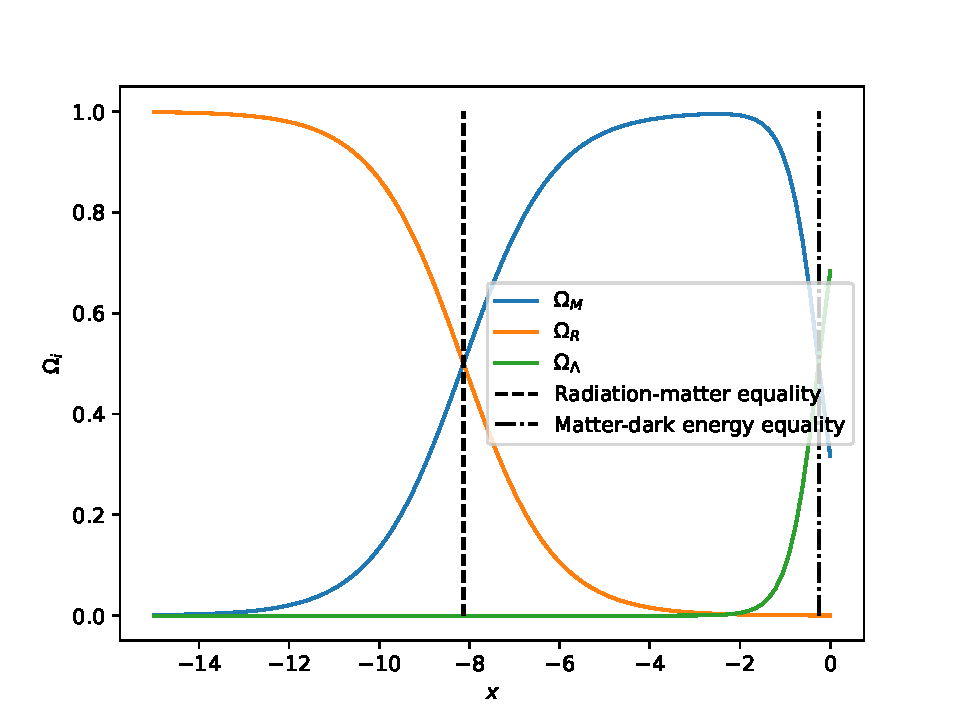
\includegraphics[width=\hsize]{figures/Omegas.pdf}
  \caption{Evolution of the densities of the components of the Universe as a function of the logarithm of the scale factor, where the density of matter, radiation and dark energy are shown, respectively, in blue, orange and green. The black vertical lines show the radiation-matter (dashed) and matter-dark energy (dot-dashed) equalities. In the beginning, radiation dominates; in between the two vertical lines, matter dominates; and, closer to today, dark energy dominates.}
     \label{fig:Omegas}
\end{figure}

\begin{figure}[ht]
\centering
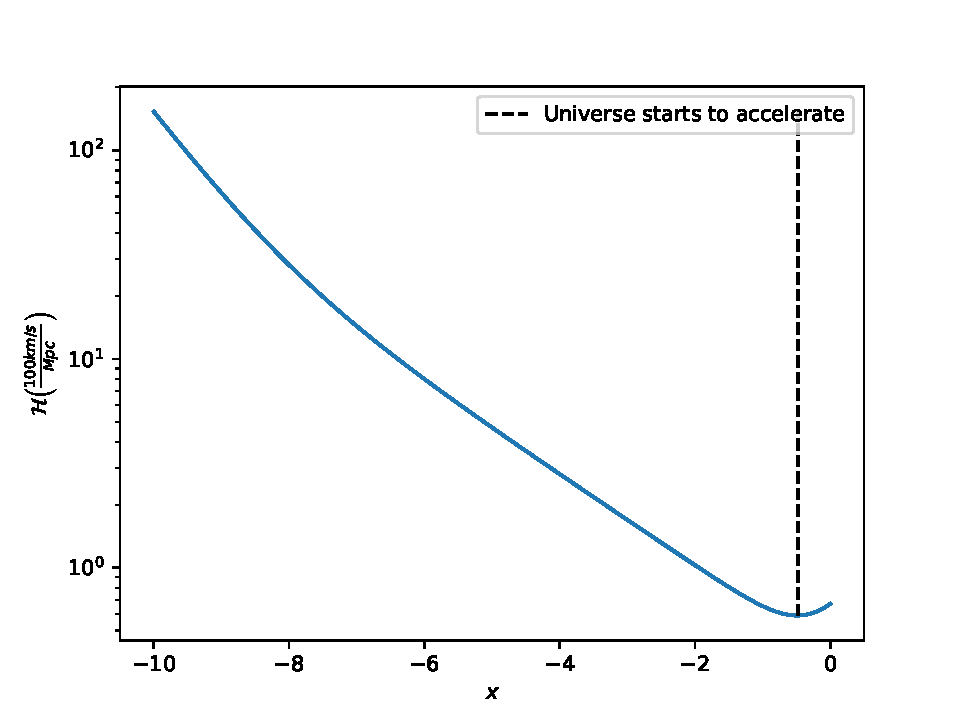
\includegraphics[width=\hsize]{figures/Hp.pdf}
  \caption{Scaled Hubble parameter as a function of the logarithm of the scale factor (blue). The black vertical dashed line represents the point where the Universe starts to accelerate.}
     \label{fig:Hp}
\end{figure}

\begin{table*}[ht]
\caption{Times of relevant events in Background Cosmology history.}             
\label{table:times}      
\centering          
\begin{tabular}{l l l l}     % 7 columns 
\hline\hline       
                      % To combine 4 columns into a single one 
& Logarithm of scale factor $x$      & Redshift $z$     & Cosmic time $t$ (Gyr)\\ 
\hline                    
Radiation-Matter Equality   & -8.1319  & 3400.3  & 5.1029 $\times 10^{-5}$ \\
Matter-Dark Energy Equality & -0.25582 & 0.29152 & 10.371                 \\
Universe starts to accelerate ($\ddot a = 0$)               & -0.47941 & 0.61513 & 7.8234\\ 
\hline                  
\end{tabular}
\end{table*}

It is also useful to look at the derivatives of $\mathcal H$ as well as the conformal time, in Figures \ref{fig:dhpdx}, \ref{fig:ddhpddx} and \ref{fig:eta}.
\begin{figure}[ht]
\centering
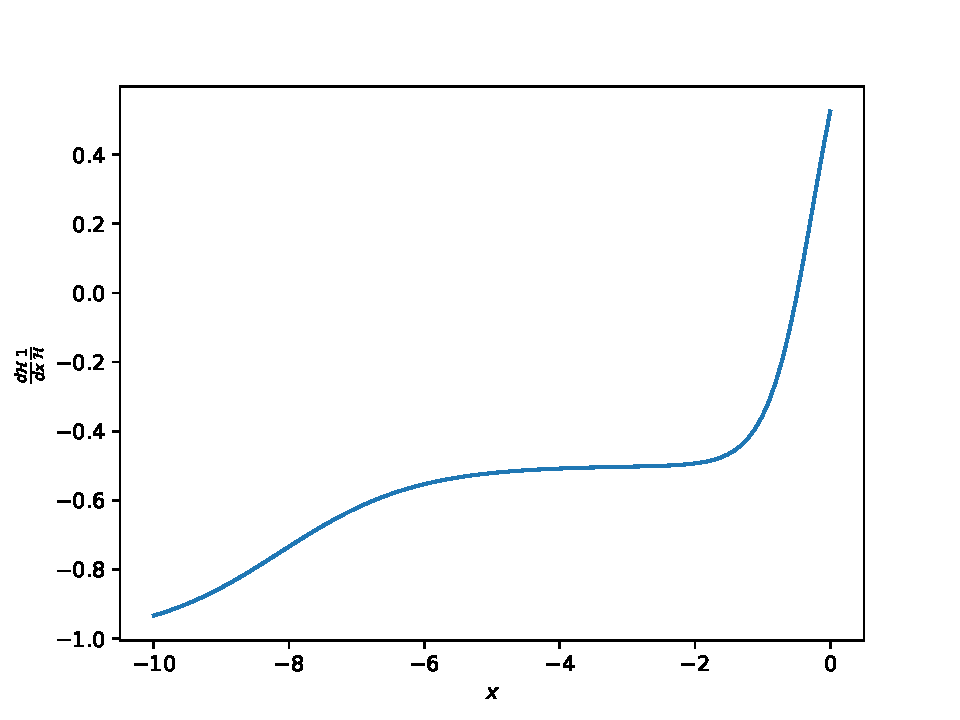
\includegraphics[width=\hsize]{figures/dHpdx_over_Hp.pdf}
  \caption{Evolution of the first derivative of the scaled Hubble parameter over the scaled Hubble parameter as a function of the logarithm of the scale factor.}
     \label{fig:dhpdx}
\end{figure}

\begin{figure}[ht]
\centering
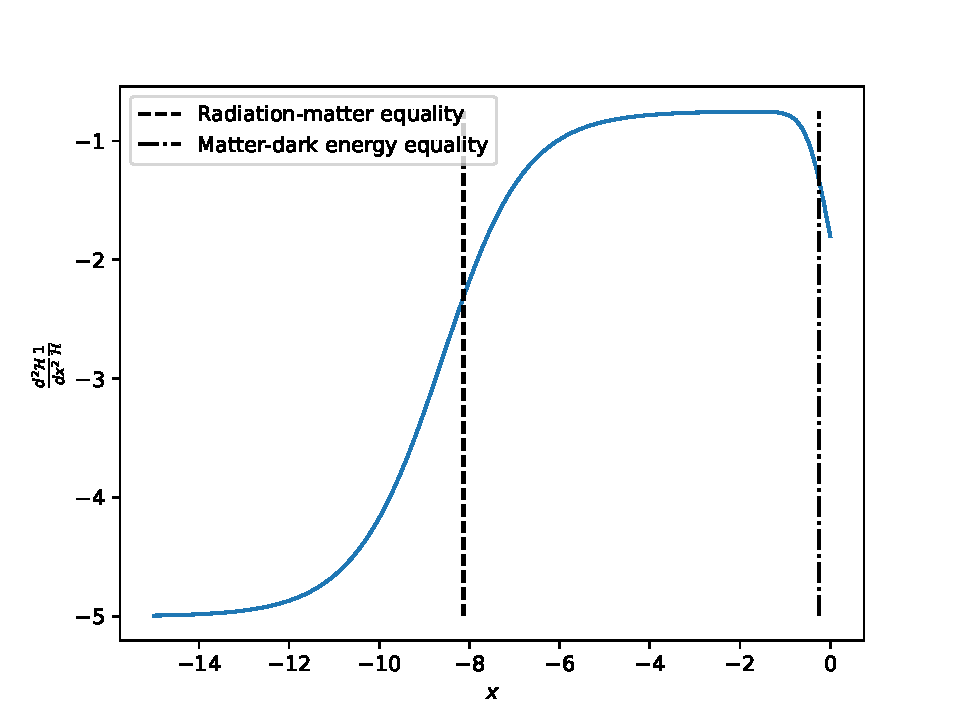
\includegraphics[width=\hsize]{figures/ddHpddx_over_Hp.pdf}
  \caption{Evolution of the second derivative of the scaled Hubble parameter over the scaled Hubble parameter as a function of the logarithm of the scale factor. \hw{Fig 4 is wrong. This is not H’’/H but seems to be just H or H’’.}}
     \label{fig:ddhpddx}
\end{figure}

\begin{figure}[ht]
\centering
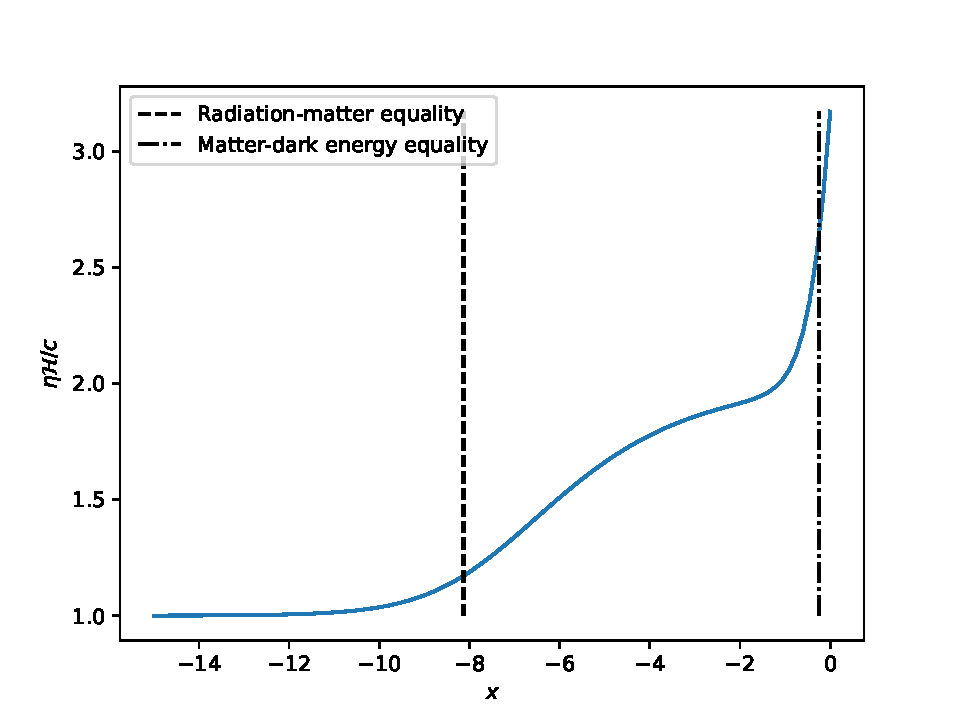
\includegraphics[width=\hsize]{figures/etaHp_over_c.pdf}
  \caption{Evolution of the conformal time times the scaled Hubble parameter as a function of the logarithm of the scale factor.}
     \label{fig:eta}
\end{figure}

As a sanity check, it is also good to look at the trends in the conformal and cosmic times in Figures \ref{fig:eta} and \ref{fig:t}. As expected, they both have an upwards trend. Additionally, we can calculate that the conformal time of today ($a = 1 \Rightarrow x = 0$) is 14.192 Gpc.

\begin{figure}[ht]
\centering
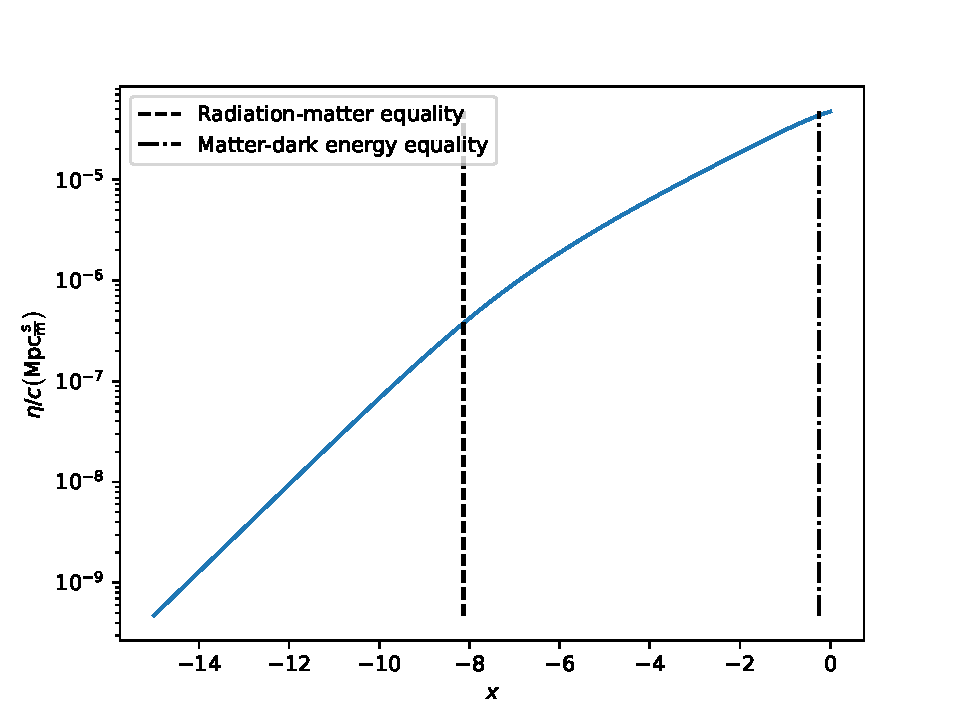
\includegraphics[width=\hsize]{figures/eta_over_c.pdf}
  \caption{Conformal time as a function of the logarithm of the scale factor. \hw{Fig 6 Missing units on y-axis.}}
     \label{fig:eta}
\end{figure}

\begin{figure}[ht]
\centering
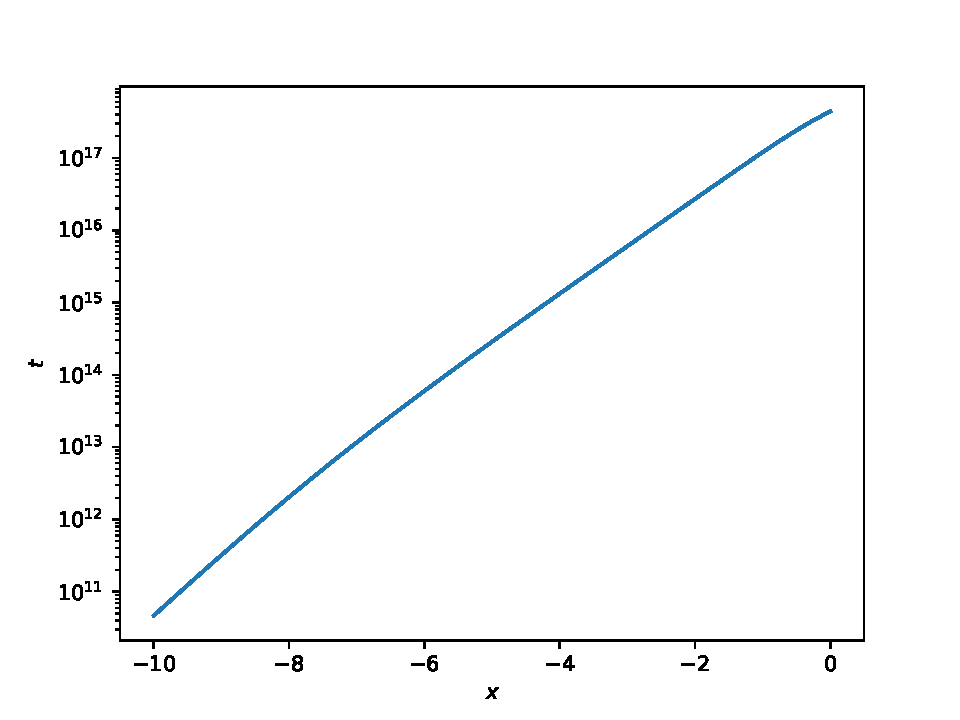
\includegraphics[width=\hsize]{figures/t.pdf}
  \caption{Cosmic time as a function of the logarithm of the scale factor. \hw{Fig 7 Missing units on y-axis.}}
     \label{fig:t}
\end{figure}

An interesting result is comparing our model to the data from \cite{Betoule_2014} by looking at the luminosity distance measure in Figure \ref{fig:dL}.

\begin{figure}[ht]
\centering
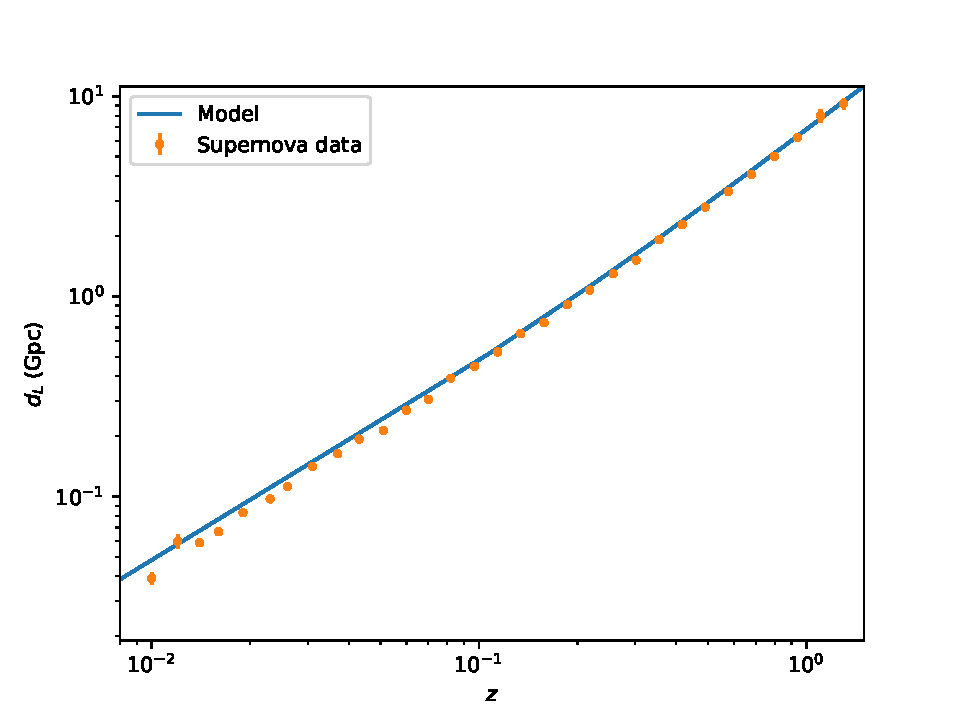
\includegraphics[width=\hsize]{figures/dL.pdf}
  \caption{Luminosity distance as a function of the logarithm of the scale factor. Our model is represented as the blue curve and the date is represented as the orange circles with their respective error bars. \hw{Fig 8 Hard to see if the line goes through the data points or now. Here scaling the line and data (e.g. $d_L$ / z or similar) can help.}}
     \label{fig:dL}
\end{figure}

We now want to take a look at our MCMC fits. In Figure \ref{fig:fitting}, we can see the 1$\sigma$ prediction for the value of the densities of matter and dark energy. Our predictions agree with a flat Universe. Lastly, we have a 1$\sigma$ posterior prediction for the Hubble constant as shown in Figure \ref{fit:hist} around 70 km s$^{-1}$ Mpc$^{-1}$, which does not span to the Planck best-fit value. This might be because our model is not intricate enough yet to describe the Universe. However, it is still fairly close to the values predicted by different recent experiments.

\hw{“This might be because our model is not intricate enough yet to describe the Universe. However, it is still fairly close to the values predicted by different recent experiments.”  See \url{https://cmb.wintherscoming.no/theory_background.php#tension}}

\begin{figure}[ht]
\centering
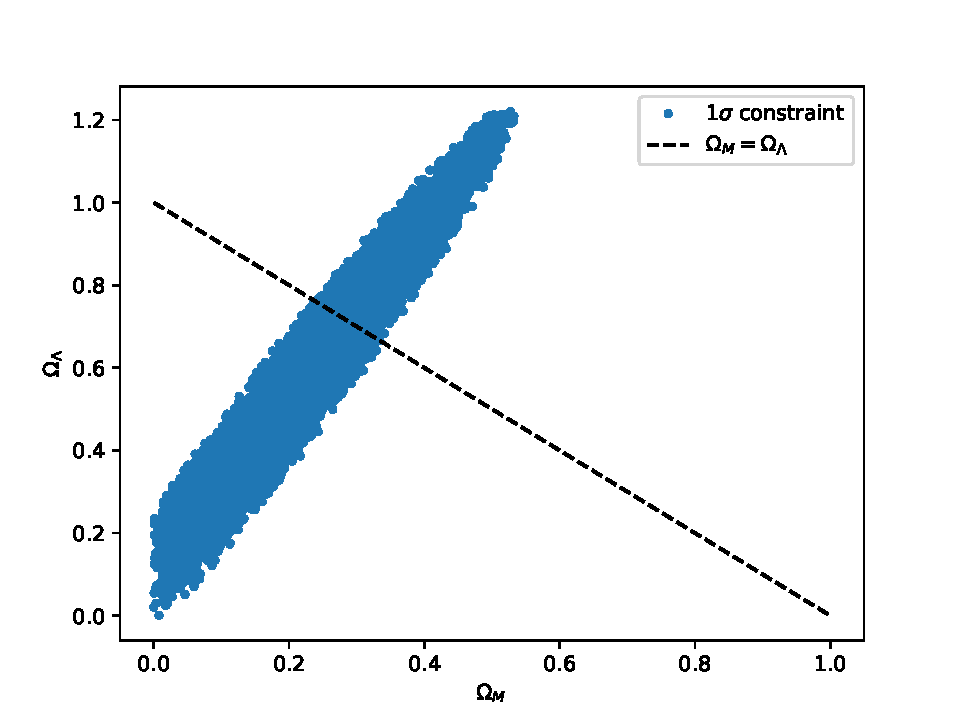
\includegraphics[width=\hsize]{figures/fitting.pdf}
  \caption{1$\sigma$ prediction for the densities of matter and dark energy. \hw{Fig 9 is wrong due to the bug mentioned below (line 201). You get that OmegaLambda = 0 is allowed which it should not be.}}
     \label{fig:fitting}
\end{figure}

\hw{Describe better what is shown in the caption.}

\hw{Fig 3 and 4. Here you can compare this to analytically expected values in different regimes to validate your results.}

\begin{figure}[ht]
\centering
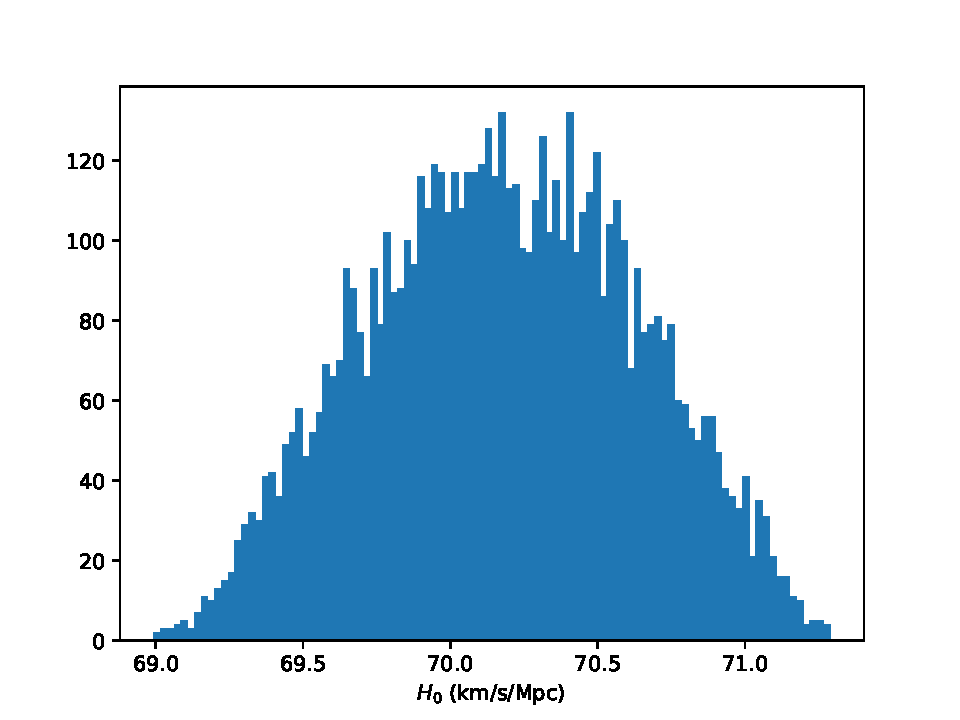
\includegraphics[width=\hsize]{figures/histogram.pdf}
  \caption{1$\sigma$ prediction for the Hubble constant.}
     \label{fit:hist}
\end{figure}

\subsection{Recombination History}

Figure \ref{fig:Xe-Saha} shows the fractional electron density $X_e$ over time $x$. The blue line describes the Saha solution. The orange line describes the full solution, starting by solving the Saha equations, until $X_e$ reaches 0.99, and then by solving the Peebles ODE. The Saha equations give a solution that falls off much faster than what is verified by experiments, and thus the need arises for the Peebles solution. Furthermore, we show the times of the last scattering and recombination, which happen almost simultaneously. Saha also predicts that recombination happens earlier than Peebles, consequence of the $X_e$ curve falling off faster. Around -8.5 to -8 and -8 to -7.5, we can see the recombination stages of singly and doubly ionised helium, following by that of hydrogen.

As we tend towards freeze-out, we can see that the fractional electron density is stable since recombination at around $0.00026736$, when ionisation is not considered.

\begin{figure}[ht]
    \centering
    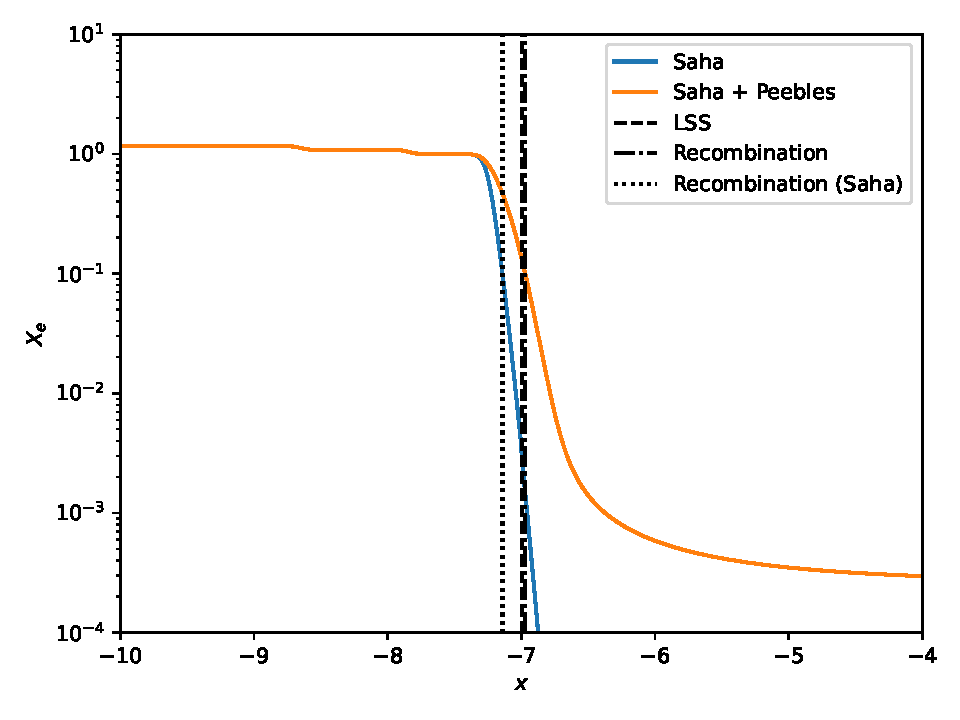
\includegraphics[width=\hsize]{report/figures/Xe.pdf}
    \caption{Fractional electron density $X_e$ given by the Saha equations (blue) and by full solution (orange) over time. Relevant times are marked in black vertical lines: the last scattering surface (surface) (LSS) (dashed),  recombination (dot-dashed) and recombination when calculated according only to the Saha equations (dotted). Reionisation is not used for the curves represented in this plot.}
    \label{fig:Xe-Saha}
\end{figure}

Calculating the fractional energy density until today, we find Figure \ref{fig:Xe-reion}. The helium recombination drop-offs are more obvious in this plot, as it is in linear scale on the y-axis, as opposed to the previous plot, which was in logarithmic scale and aimed to look at the differences between the full solution and the Saha solution. We can also see that the electron density rises again after reionization, both for hydrogen and helium. As such, we are able to identify three matter epochs: plasma (green), neutral hydrogren and helium (red) and neutral and ionised species (purple), which are separated by recombination and ionisation. These times are listed in Table \ref{table:times-rec}.

\begin{figure}[ht]
    \centering
    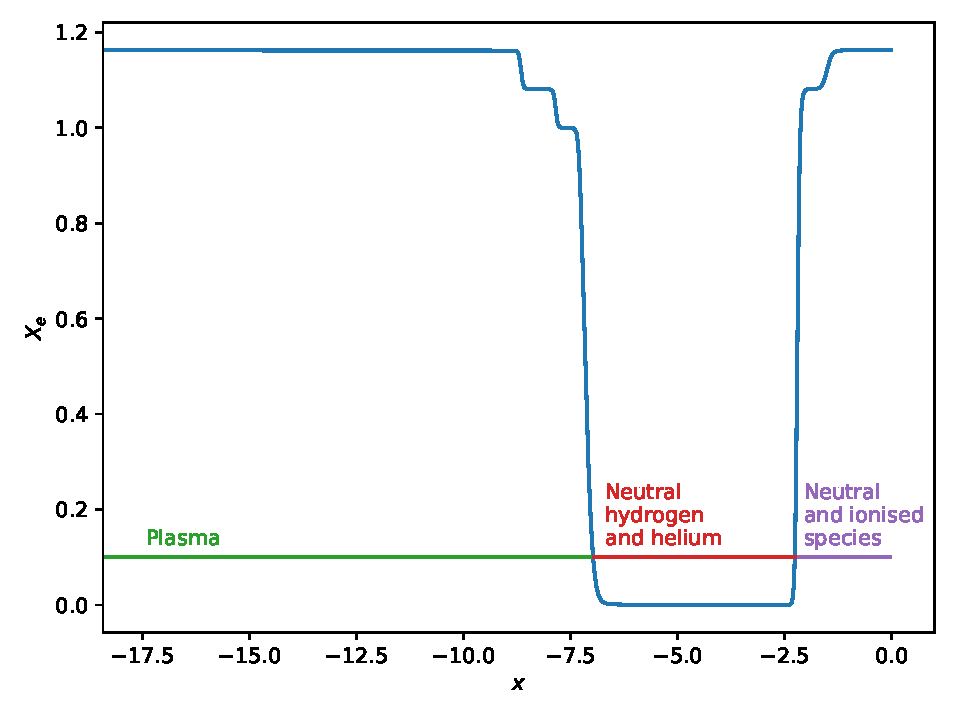
\includegraphics[width=\hsize]{report/figures/Xe-reion.pdf}
    \caption{Fractional electron density $X_e$ (blue) over time. The dominating matter epochs are shown by the horizontal lines: plasma (green) dominates in the early Universe, neutral hydrogen and helium (red) dominate after recombination and before reionization, and a mixture of neutral and ionised species (purple) dominate after reionization.}
    \label{fig:Xe-reion}
\end{figure}

\begin{table*}[ht]
\caption{Times of relevant events in recombination history.}             
\label{table:times-rec}      
\centering          
\begin{tabular}{l l l l}     % 7 columns 
\hline\hline       
                      % To combine 4 columns into a single one 
& Logarithm of scale factor $x$      & Redshift $z$     & Cosmic time $t$ (Myr)\\ 
\hline                    
Last scattering   & -6.9901  & 1084.8  & 0.37478 \\
Recombination & -6.9701 & 1063.3 & 0.38758                 \\
Recombination (according to Saha) & -7.1403 & 1260.9 & 0.29069\\
Reionisation & -2.2014 & 8.0377 & 633.34\\
\hline                  
\end{tabular}
\end{table*}

The optical depth $\tau$ (blue) and its first (orange, times -1) and second (green) derivatives w.r.t. $x$ over time $x$ are shown in Figure \ref{fig:tau}. We can see that the optical depth in the early Universe is very large, meaning the photon-baryon plasma is an optically thick medium, where no light can be transmitted. The time of the last scattering is pointed out by the black vertical dashed line, defined by $\tau=1$. After this point, the optical depth is lower than one stable until reionisation, and thereafter it starts decreasing again, meaning photons are able to travel through the medium since recombination until today.

\begin{figure}[ht]
    \centering
    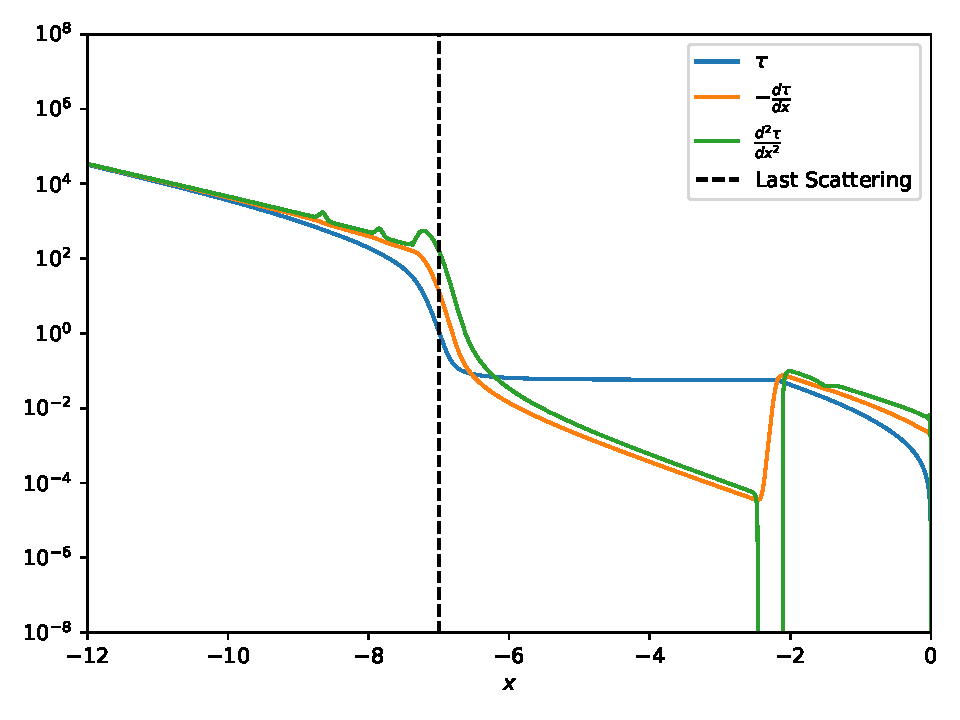
\includegraphics[width=\hsize]{report/figures/tau.pdf}
    \caption{Optical depth $\tau$ (blue), as well as its first (orange) and second (green) derivatives w.r.t. $x$ over time. The time of the last scattering is pointed out by the black vertical dashed line.}
    \label{fig:tau}
\end{figure}

One last useful visualization is Figure \ref{fig:gtilde}, where we look at the visibility function $\tilde g$ (blue) and its first (orange) and second (green) derivatives w.r.t. $x$ over $x$, with each curve normalized. $\tilde g$ peaks around the same time as recombination, and then there is a smaller peak around reionisation.

\begin{figure}[ht]
    \centering
    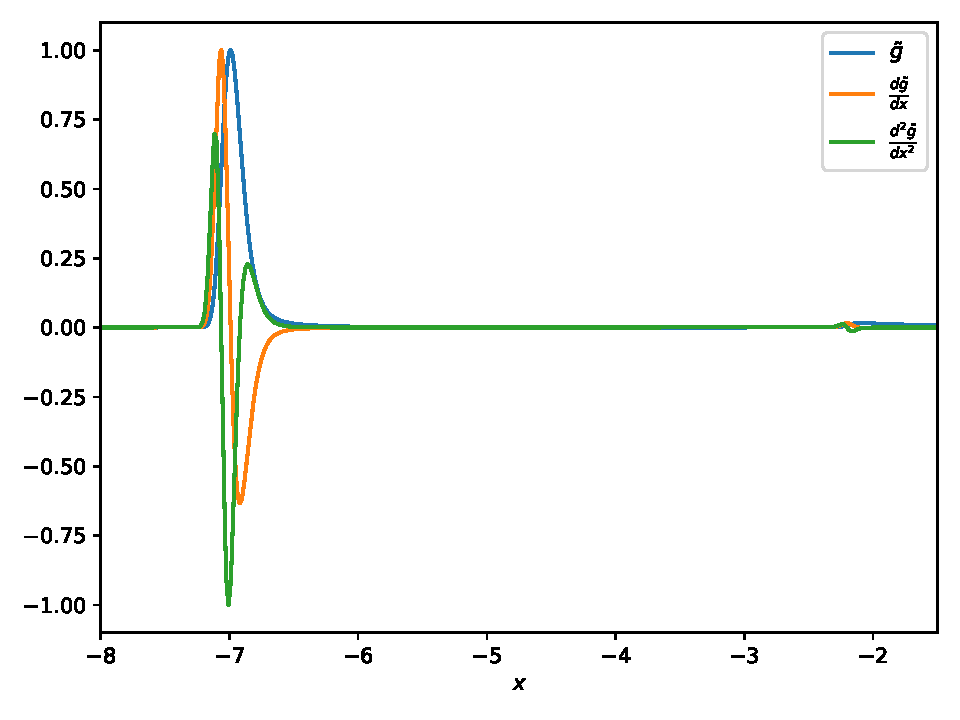
\includegraphics[width=\hsize]{report/figures/gtilde.pdf}
    \caption{Visibility function $\tilde g$ (blue) and its first (orange) and second (green) derivatives w.r.t. $x$ over time. All are normalized.}
    \label{fig:gtilde}
\end{figure}

We can calculate the distance a sound-wave can propagate through the photon-baryon plasma from the Big Bang until recombination by calculating the sound-horizon at decoupling, which is then $r_s = 144.84$ Mpc.

\section{Conclusions}

\subsection{Background Cosmology}
We have simulated the Universe from the CMB until the present day. We present various results and compare them to experimental data which validates our model to reasonable accuracy. In particular we find that the radiation-matter and matter-dark energy equality happen, respectively, at $x = -8.1319$ and $x = -0.25582$, whereas the Universe starts to accelerate at $x=-0.47941$.

\subsection{Recombination History}

We have simulated the recombination and reionisation events, considering that the neutral atoms era is made up of only hydrogen and helium. For this, we calculated the electron fraction using the Saha and Peebles equations, which then gives us the optical depth which in turn gives us the visibility function. We find that decoupling happens around $x=-7$ and reionisation around $x=2.2$. The fractional electron density $X_e$ at freeze-out is 0.00026736. The sound-horizon at decoupling $r_s$ is 144.84 Mpc.

%\begin{acknowledgements}

%\end{acknowledgements}

% WARNING
%-------------------------------------------------------------------
% Please note that we have included the references to the file aa.dem in
% order to compile it, but we ask you to:
%
% - use BibTeX with the regular commands:
%   \bibliographystyle{aa} % style aa.bst
%   \bibliography{Yourfile} % your references Yourfile.bib
%
% - join the .bib files when you upload your source files
%-------------------------------------------------------------------

\bibliographystyle{aa}
\bibliography{report/references}

\end{document}
